\section{Dominoes}

The objective is to find out where the complexity lies in the Tetris. To contribute something in this matter we will study Tetris with dominoes. From the above results it has been seen that adding more complexity in the set of pieces makes it more complicated.

Focusing on 2-\textsc{tris}, Tetris with dominoes, will help in our goal. As it can be seen in Table~\ref{tab:tt}, the variation 2-\textsc{tris-NoRotation} \clearing\ is in \npc and the only domino's problem closed.

\vspace{10px}
We will first explore two sub problems of these. We will consider the case in which all dominoes appear vertically and the case in which all pieces appear horizontally.

Then ....

\subsection{Tetris with vertical dominoes}

Using the introduced notation, the problem is $\textsc{Tetris-NoRotation}\lbrack \VD \rbrack $ both  \clearing\  and \survival. The input consist of sequence of vertical dominoes and an arbitrary sized $n \times m$ board in a contractible configuration. The initial state function used in this variation differs since the default on the initial orientation, since the pieces must come in vertical orientation.

\subsubsection{Constructible board configurations}

First we will to characterize the constructible boards with $\VD$ pieces without rotation by exploring the configuration starting from an empty board. 

Vertical dominoes consist of two vertical adjacent cells, so for an empty board any trajectory fixes the piece in the bottom row, filling $\cell[1][i]$ and $\cell[2][i]$ cells for any $1 \leq i \leq m$. The next domino can either go to an empty column or to the one before. Placing the first $m$ dominoes in unfilled columns clears the two lowest rows, and consequently the board. When a domino is placed in a non-empty column $i$, the $\cell[3][i]$ and $\cell[4][i]$ are filled, and so on, util a $\VD$ is placed in the last unfilled column. When this happens the two lowest rows are cleared and the process continues. 

So we can represent a reachable configuration of a given $n \times m$ board $B$ with a sequence of $m$ integers $(a_1, \dots, a_m)$, where

$$0 \leq a_i \leq \lceil \frac{n}{2} \rceil, \;\;\;   \forall i = 1,\dots, m$$

and $\exists i$ such that $a_i = 0$ (an empty column), with the following mapping: 

$$
\cell = \begin{cases}
   \text{filled}  & \text{if } i \leq  2a_j  \\
   \text{empty}   & \text{if } i >  2a_j
\end{cases}
$$

Each $a_i$ counts the number of vertical pieces placed in the column $i$. For example, in a $10 \times 6 $  board, the sequence $(1,2,0,4,2,3)$ defines the configuration in 
\ref{dom:vconf}.

\begin{figure}[ht]
  \centering
  \begin{subfigure}[b]{0.2\textwidth}
    \centering
    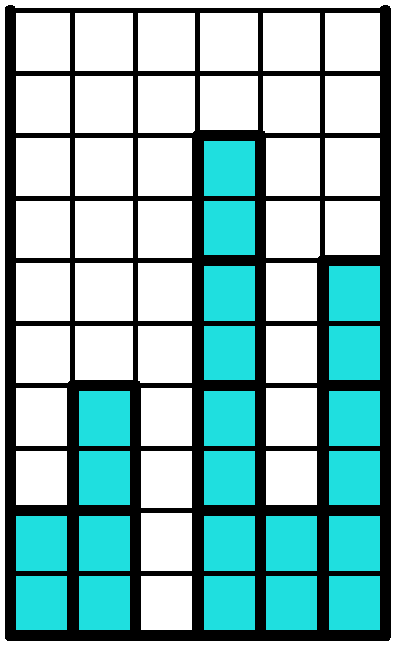
\includegraphics[width=0.9\textwidth]{pictures/dominoes/vertical_configuration.pdf}
    \caption{}
  \end{subfigure}
  \begin{subfigure}[b]{0.2\textwidth}
    \centering
    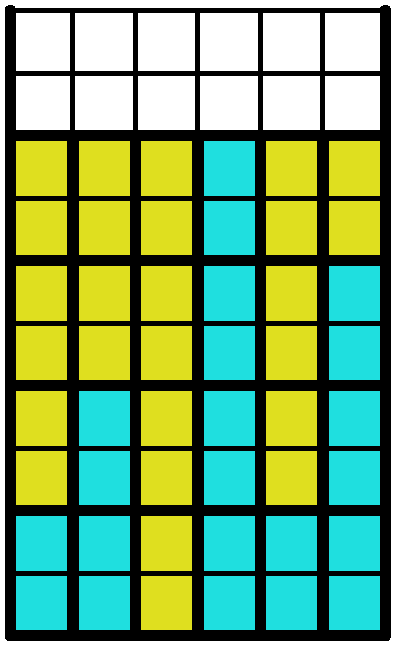
\includegraphics[width=0.9\textwidth]{pictures/dominoes/vertical_configuration_filled.pdf}
    \caption{}
  \end{subfigure}
    \caption{The $10 \times 6 $ board configuration represented by the sequence $(1,2,0,4,2,3)$, in yellow the 13 dominoes needed to clear the board.}
  \label{dom:vconf}
\end{figure}

\subsubsection{Cleaing}

In this decisional problem the input is a sequence of $k$ vertical dominoes and an $n \times m$ board with an initial configuration, that can be represented by the sequence $(a_1, \dots, a_m)$ as before. The question is: \emph{Is ther a way to clean the board after placing the $k$ pieces?}

\begin{theorem} 
$\textsc{Tetris-NoRotation}\lbrack \VD \rbrack $ \clearing\ is in \pp.
\label{dom:no-rot-vd}
\end{theorem}
\begin{proof}
    Let $B = (a_1, \dots, a_m) $ be the board representation and $k$ the length of the sequence of vertical dominoes. For every constructible board there is an empty column, so the strategy consists on placing each piece in an arbitrary empty column. 

    All the empty cells under the lowest empty row need to be filled to clean the board. Let $a_{\max}$ be the max in the board representation. Since we fill cells with dominoes, the number of dominoes $k_{\min}$ needed to clean the board is:
    $$ k_{\min} = \sum_{i = 1}^m \left( a_{\max} - a_i \right) $$

    If $k < k_{\min}$ we can't clear the board. If $k =  k_{\min}$ we can clear the board. And when $k > k_{\min}$, we can clean the board if after placing $k_{\min}$ dominoes the number of remaining pieces is a multiple of the board width, $k - k_{\min} \equiv 0 \mod m$. Since all the computations can be done in polyatomic time in respect of the input, the problem is in \pp.
\end{proof}

For boards with an even number of rows all pieces always fit inside the board. For an odd number of rows, dominoes could be placed in the top row with half of the domino inside the board and half outside. If we allow this, by changing the \emph{fix} function, the result would be the same since the same strategy works. The Figure~\ref{dom:vconf} shows, in yellow color, how the number of pieces needed to clean the board.

\subsubsection{Survival}

With the same input, the objective is to do not lose. The last proof provides a strategy to survive indefinitely. So for any number of pieces $k$ there is a way to avoid losing. Hence:
\begin{theorem} 
$\textsc{Tetris-NoRotation}\lbrack \VD \rbrack $ \survival\ is in \pp.
\end{theorem}


\subsection{Tetris with horizontal dominoes}

As before, the problem is $\textsc{Tetris-NoRotation}\lbrack \HD \rbrack $ both \clearing\ and \survival. Placing a horizontal domino fills two adjacent cells in one row or clears the row, so each domino placed can be tracked until the row is cleared. Hence, for any initial constructible configuration, the filled cells can be uniquely grouped into dominoes. We can refer to dominoes instead of filled cells.

Also, in any constructible board each row has an even number of filled cells, so when the board width is odd row can be cleared. In this scenario the board can be cleared if the input consists on an empty board and an empty sequence of pieces. From now and on we assume the board has an even number of columns. Let $B$ be a board with $m$ columns. Let's divide the board in $m/2$ \emph{buckets}, a pair of consecutive columns. Then:

\begin{lemma0}   
    Not placing a domino inside a bucket makes the row unclearable.
\end{lemma0}
\begin{proof}
    Let $r$ be a row containing some dominoes. When a domino is placed in a bucket it divides the row into two parts: the cells on the left side of the domino and the ones on the right. Both parts of even length, and containing an even number of filled cells.

    In the other case the two parts have an odd length but containing an eaven number of filled cells, making them impossible to clean
    since there's no way to add an odd number of cells by placing dominoes.
\end{proof}

For example, in the Figure~\ref{dom:buckets}, the second piece occupies the second and the third bucket, making the row un-clearable. 

\begin{figure}[h]
    \centering
    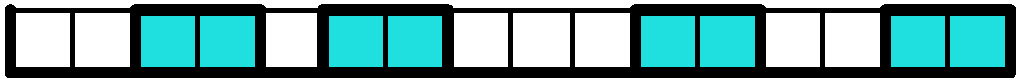
\includegraphics[width=0.2\textwidth]{./pictures/dominoes/buckets.pdf}
    \caption{A board with one partially filled row.}
    \label{dom:buckets} 
\end{figure}


We now can prove both clearing and survival problems.

\begin{theorem}
    $\textsc{Tetris-NoRotation}\lbrack \HD \rbrack $ \clearing\ is in \pp.
\end{theorem}
\begin{proof}


    The input is an $n \times m$ input board $B$, filled with a construable configuration, and sequence of $k$ dominoes $\HD$. If $m$ is odd then the board can't be cleared if $k > 0$ or the initial board isn't empty. 

    When $m$ is even we first need to check if the board is clearable. If there's only one row, checking that the row has been built by placing each piece inside a bucket determines if the row is clearable. When the board has more than one row the same happens. 

    We first group in pieces the filled cells of each row from the initial board. This can always be done because there's no way to clean \emph{"half"} piece. Then we check if each piece is placed inside a bucket. If some piece isn't placed inside a bucket the board can't be cleared. We can compute this in $\mathcal{O}(n\cdot m)$.

    Now the board can be represented with a sequence $(a_1, \dots, a_{m/2})$ of $m/2$ numbers each representing the number of dominoes placed in each bucket.

    $$
    \cell = \begin{cases}
        \text{filled}  & \text{if } i \leq  a_{2j}  \\
        \text{empty}   & \text{if } i >  a_{2j}
    \end{cases}
    $$

    With some $a_i = 0$. Let $a_{\max} = \max \{a_1, \dots a_{m/2}$ \} be the maximum of the sequence. The minimum number of pieces needed to clear the board is:

    $$ k_{\min} = \sum_{i = 1}^{m/2} (a_{\max} - a_i )$$

    If $k < k_{\min}$ the board can't be cleared. If $k = k_{\min}$ the board can be cleared. When $k > k_{\min}$ the board can be cleared if $ k - k_{\min} \equiv 0 \mod m / 2$, sine the remaining pieces have to leave the board empty by filling rows.
\end{proof}

\begin{figure}[ht]
  \centering
  \begin{subfigure}[b]{0.3\textwidth}
    \centering
    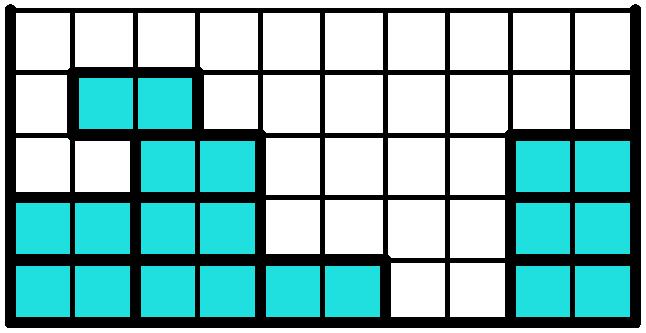
\includegraphics[width=0.9\textwidth]{pictures/dominoes/horitzonatl_configuration_1.pdf}
    \caption{}
  \end{subfigure}
  \begin{subfigure}[b]{0.3\textwidth}
    \centering
    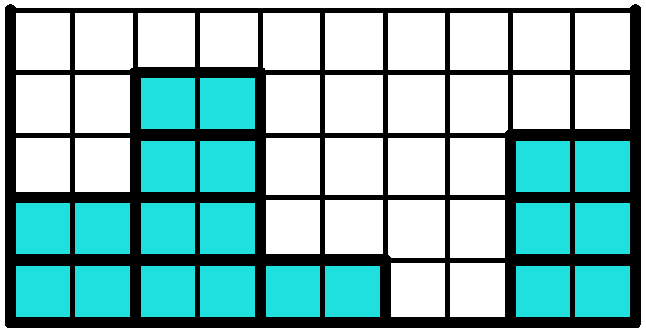
\includegraphics[width=0.9\textwidth]{pictures/dominoes/horitzonatl_configuration_2.pdf}
    \caption{}
  \end{subfigure}
  \begin{subfigure}[b]{0.3\textwidth}
    \centering
    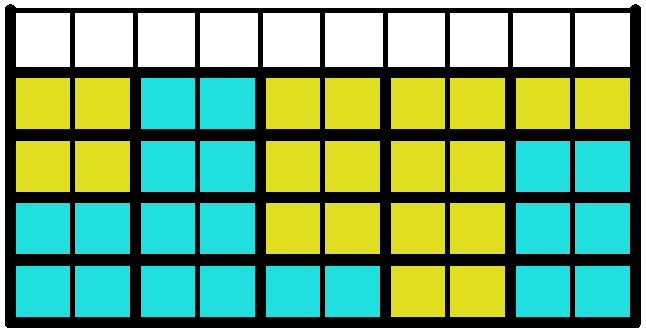
\includegraphics[width=0.9\textwidth]{pictures/dominoes/horitzonatl_configuration_3.pdf}
    \caption{}
  \end{subfigure}
  \caption{Some board configurations. In (a) the board can't be cleared because the topmost domino is placed between the first and the second bucket. In (b) the board is represented by the sequence $(2,4,1,0,3)$, it can be cleared. The minimum number of pieces to clean the board is 10, this pieces appear in yellow in (c).}
  \label{dom:horitzonatl_configuration}
\end{figure}

Figure~\ref{dom:horitzonatl_configuration} shows some examples of the above prof. Next follows the \survival. In this scenario the goal is to find a strategy to survive indefinitely. Before the result, we need a lemma about floating dominoes. A floating domino is a domino that the two below cells are unfilled.  

\begin{lemma0}
In \( \textsc{Tetris-NoRotation}\lbrack \HD \rbrack \), any floating domino (yellow) must have two dominoes (blue) placed to the left and right of the unfilled cells directly below it:

\[
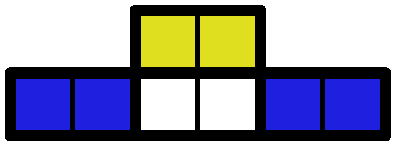
\includegraphics[scale=0.3]{./pictures/dominoes/proff-floating/foating.pdf}
\]
\end{lemma0}

\begin{proof}
Let \( B \) be an \( n \times m \) board containing a floating domino (yellow). For a floating domino to exist, the width \( m \) of the board must be even, as this piece cannot be fixed in its current position without further row clearing. Thus, we assume some rows must be cleared for the domino to be in this state. Let \( B_0, B_1, \dots, B_k = B \) represent the sequence of boards that transitions from an empty board \( B_0 \) to the board \( B_k \), which contains the floating domino. Without loss of generality, assume \( B_k \) is the first board in the sequence to include a floating domino.

A floating domino cannot result from adding a domino that does not clear a row. Therefore, \( B_k \) must be obtained by adding a domino to \( B_{k-1} \) in such a way that it clears a row. Let \( r \) denote the row cleared in \( B_{k-1} \). Clearing row \( r \) modifies only the neighboring rows \( r-1 \) and \( r+1 \). Cells below \( r \) do not become floating as a result of removing row \( r \). Consequently, the added domino must lie on row \( r \) in \( B_{k+1} \).



Thus, the floating domino in \( B_k \) must occupy positions \( d_k = (\cell[r], \cell[r][j+1]) \), and it must originate from a domino in \( B_{k-1} \) occupying \( d_{k-1} = (\cell[r+1], \cell[r+1][j+1]) \). In \( B_{k-1} \), the cells directly below \( d_{k-1} \) in row \( r \) are filled by dominoes that are not floating. This leads to four possible configurations of dominoes in \( B_{k-1} \) around \( d_{k-1} \):

\[
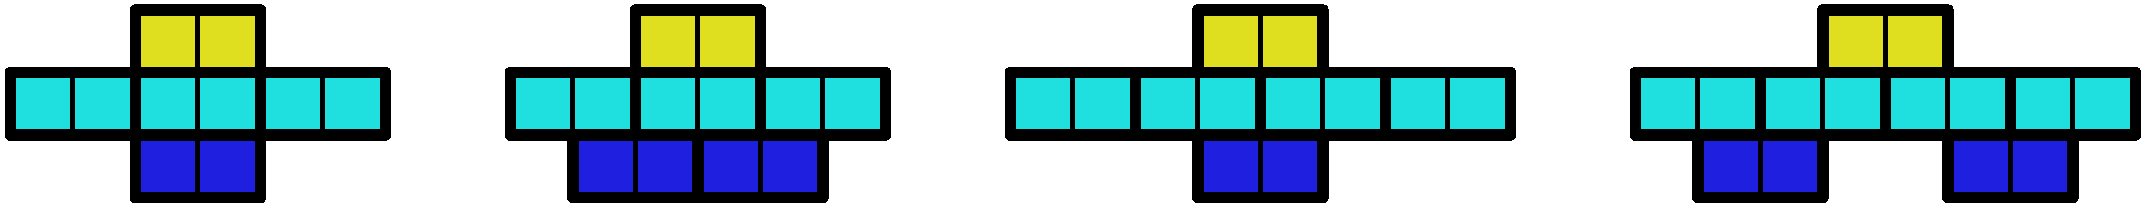
\includegraphics[scale=0.3]{./pictures/dominoes/proff-floating/2.pdf}
\]

Among these scenarios, only the last configuration results in a floating domino appearing in \( B_k \) after clearing row \( r \). In this case, the two cells directly below the floating domino (yellow) in \( B_k \) must each be part of dominoes extending left and right, ensuring the stability of the structure. Therefore, the floating domino requires two supporting dominoes (blue) to the left and right of the unfilled cells below it.
\end{proof}

Moreover, this lemma implies that in any constructible configuration, there cannot be completely floating blocks, blocks whose lower corners aren't touching any domino.

\begin{theorem}
    $ \textsc{Tetris-NoRotation}\lbrack \HD \rbrack $ \survival\ is in \pp.
\end{theorem}
\begin{proof}
    
If a given board \( B \) contains a clearable row, we can survive indefinitely by first clearing this row and then continuing to place pieces to refill the topmost row. If no such row exists---for instance, on a board with odd width---there exists a maximum number \( k_{\max} \) of dominoes that can be placed before a loss becomes inevitable. Thus, if the input length \( k \) is less than or equal to \( k_{\max} \), survival is possible; otherwise, it is not. The following procedure checks if any row can be cleared and, if not, computes \( k_{\max} \).

Horizontal dominoes fit naturally in a row, so maximizing the number of dominoes placed on the board \( B \) requires maximizing their placement in each row. To avoid blocking further placements, the board is filled from the bottom to the top. Within a row, a \emph{hole} is defined as a set of contiguous empty cells bounded by filled cells or the board's edges. 

% More formally, for row \( r \), a \emph{hole} is a segment:
%
% \[h^r_{j_1,j_2} = \{\cell[r][j_1], \cell[r][j_1+1], \dots, \cell[r][j_2]\}\]
%
% where all cells in \( h \) are empty, and the boundary cells \( \cell[r][j_1-1] \) and \( \cell[r][j_2+1] \) are either filled or lie outside the board.

To maximize the number of dominoes in the board, each row's holes must be filled as completely as possible. This reduces the problem of filling the entire board to the simpler task of optimally filling individual row holes. By systematically filling holes from the bottom-most row upwards, we ensure the greatest number of dominoes are placed without causing unresolvable blocking.

Let \(h = \{\cell[r][j_1], \cell[r][j_1+1], \dots, \cell[r][j_2]\}\) be a hole in row $r$ from column $j_i$ to $j_2$, where all cells in \( h \) are empty, and the boundary cells \( \cell[r][j_1-1] \) and \( \cell[r][j_2+1] \) are either filled or lie outside the board. There must be a trajectory for a domino from the top of the board to $h$ in order to place a piece inside the hole, so we only consider the reachable holes.

If two trajectories reach the same hole, all the cells between them can't be filled because this would imply the existence of completely floating cells. Figure~\ref{dom:hole-paths} shows an example. If a cell of the hole $\cell[r][j] \in h$ is below a filled cell $\cell[r+1][j]$ then $j = j_1$ or $j = j_2$ due to the previous lemma. So a hole has one of the shapes in Figure~\ref{dom:holes}

\begin{figure}[h]
    \centering
    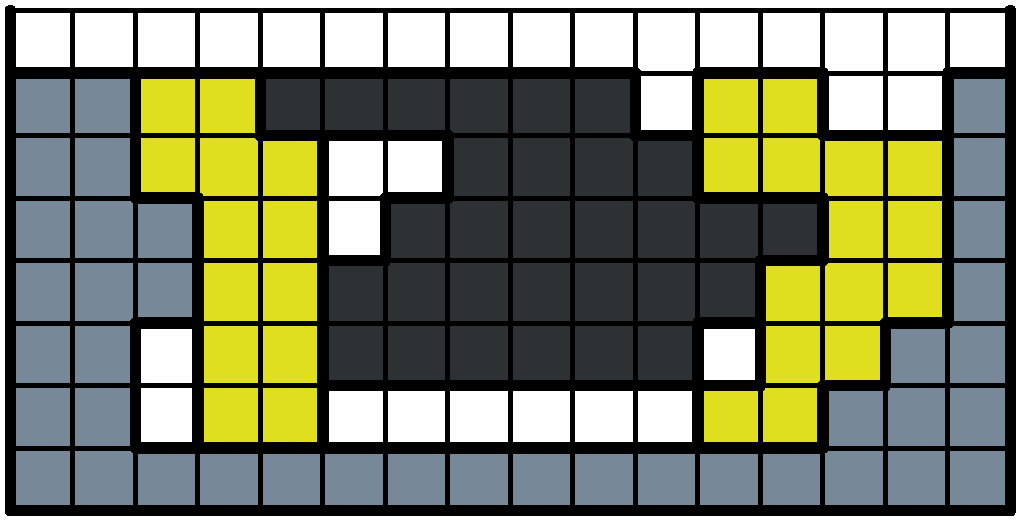
\includegraphics[width=0.4\textwidth]{./pictures/dominoes/hole-paths.pdf}
    \caption{A hole in row 2 and two paths, in yellow, that reach the hole with  filled cells (dark gary) between. }
    \label{dom:hole-paths} 
\end{figure}

\begin{figure}[ht]
  \centering
  \begin{subfigure}[b]{0.3\textwidth}
    \centering
    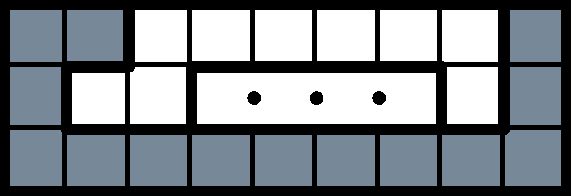
\includegraphics[width=0.9\textwidth]{pictures/dominoes/simple-hole-1.pdf}
    \caption{}
    \label{dom:hole-a}
  \end{subfigure}
  \begin{subfigure}[b]{0.3\textwidth}
    \centering
    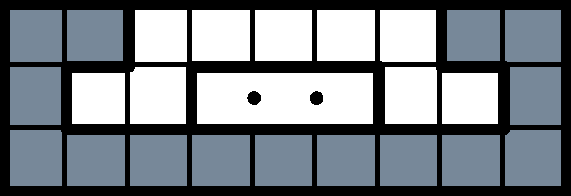
\includegraphics[width=0.9\textwidth]{pictures/dominoes/simple-hole-2.pdf}
    \caption{}
    \label{dom:hole-b}
  \end{subfigure}
  \begin{subfigure}[b]{0.3\textwidth}
    \centering
    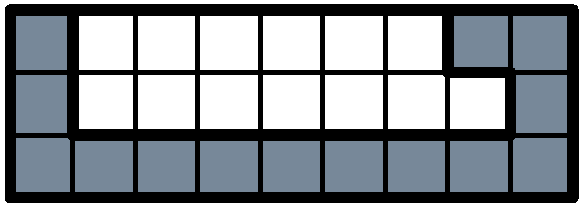
\includegraphics[width=0.9\textwidth]{pictures/dominoes/simple-hole-3.pdf}
    \caption{}
    \label{dom:hole-c}
  \end{subfigure}
    \caption{The possible shapes of a row hole.}
  \label{dom:holes}
\end{figure}

Let $l = j_2 - j_1 + 1$ the hole $h$ length. The maximin number of dominos that can be placed in  \ref{dom:hole-a} and \ref{dom:hole-c} is $h / 2$, filling completely the block if the hole lengh is even. For hole \ref{dom:hole-b} the same happens except for $l= 4$, where we can only place one domine, see Figure~\ref{dom:hole-4}.

\begin{figure}[h]
    \centering
    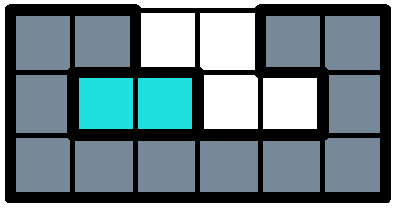
\includegraphics[width=0.18\textwidth]{./pictures/dominoes/hole-4.pdf}
    \caption{A \ref{dom:hole-b} of length 4.}
    \label{dom:hole-4} 
\end{figure}

Finally, the algorithm to decide the problem would look like:
\begin{algorithm}
\caption{}\label{euclid}
\begin{algorithmic}[1]
\Function{Tetris-NoRotation[$\HD$]}{$B,k$} \Comment{a board $B$ and $k$ dominos}
\State $k_{\max}\gets 0$

\For{row $r = 1, \dots, n$}
\State $\text{full} \gets \text{True}$
  \For{hole $h$ in $r$}
    \If{}
      \State $\text{full} \gets \text{False}$
    \EndIf
      
    \State $k_{\max} = k + l$
  \EndFor

  \If{ $\text{full}$}
    \State \return $\text{True}$
  \EndIf
\EndFor

\State \textbf{return} $k \leq k_{\max}$
\EndFunction
\end{algorithmic}
\end{algorithm}

\end{proof}


\subsection{Tetris Survival Without Rotation}

The problem  $\textsc{Tetris-NoRotation}\lbrack \VD \rbrack $ \survival\ can be formulated as: \emph{given an arbitrary sized board with an initial configuration and a sequence of $k$ dominoes, is there any way to play all the pieces while avoid losing?}. As is pointed in \cite{TT}, if there's a way to clear a single row then we can survive indefinitely with the following piece placing strategy: 

\begin{enumerate}
    \item Rotate the piece to be vertical. 
    \item Place the piece in any column with the two top cells empty.
\end{enumerate}

So to solve the problem we must show that, when the top row isn't empty, deciding if any row can be cleared is in \pp. 

\vspace{10px}

Before anything else we first define how dominoes a piece state is mapped into the board and how pieces move. A domino state $\piece[\VD][\theta][i][j][f]$ is mapped into: 

\begin{center}
\begin{equation}
\piece[\VD][\theta][i][j][f] \mapsto  \begin{cases}
    \{ \cell, \cell[i][j+1] \} &\text{if } \theta = 0^\circ\\
    \{ \cell, \cell[i-1][j] \} &\text{if } \theta = 90^\circ\\
    \{ \cell, \cell[i][j-1] \} &\text{if } \theta = 190^\circ\\
    \{ \cell, \cell[i+1][j] \} &\text{if } \theta = 270^\circ
\end{cases}
\end{equation}
\end{center}

It works like a clock. The piece position is the center and the second cell works as the clock handle. Figure~\ref{dom:mapping} shows the mapping for all orientations.

\begin{figure}[h]
    \centering
    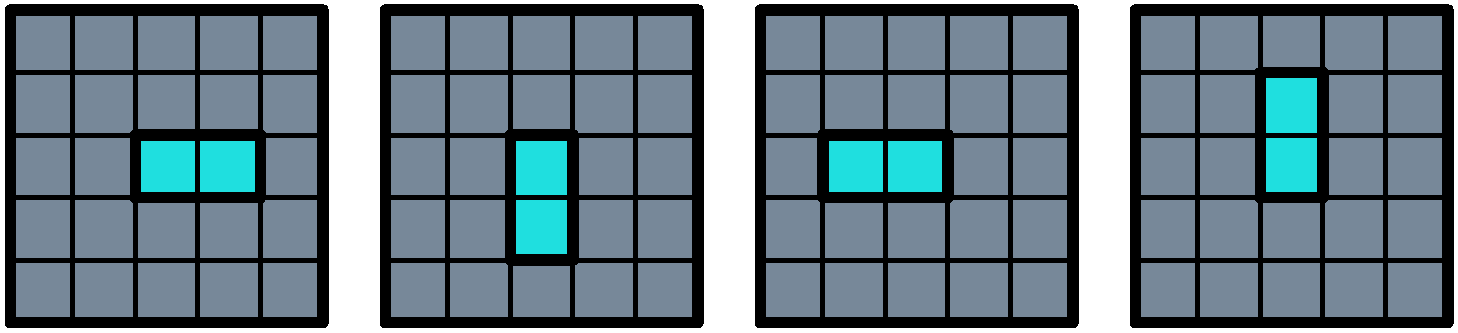
\includegraphics[width=0.6\textwidth]{./pictures/dominoes/mapping.pdf}
    \caption{The mapping of a piece placed in the center of the square and, from left to rifht, orientations $0^\circ,90^\circ,180^\circ, 270^\circ$ respectively.} 
    \label{dom:mapping} 
\end{figure}

For the moves, the usual drop and slides will be used. For the fix move we will use the \emph{partial lock rule}, witch only fixes pieces that are completely inside the board. Without this rule the strategy could be followed without the need of having the first row cleared.

For the rotation moves, the majority of modern Tetris versions use the Super Rotation System (SRS), which is the official Tetris Guideline standard for the rotation behavior of tetrominoes\cite{SRS}. When a piece is rotated, and it overlaps with a filled cell, SRS tries to place the piece in a nearby position. This is done by checking a some translations to the rotated piece. Following this idea we define a Dominoes Rotation System, DRS, with the Table~\ref{dom:rotation}.


\begin{table}[h!]
\centering
\begin{tabular}{|c || c | c || c | c ||} 
 \hline
  & \multicolumn{2}{| c ||}{ $\VD$ } & \multicolumn{2}{| c ||}{$\HD$} \\
 \hline               
 & Test 1  & Test 2 & Test 1  & Test 2 \\ 
 \hline               
 $r_+$ & $\vcenter{\hbox{
\includegraphics[scale=0.3]{./pictures/dominoes/rotation/vert_clock_1.pdf}}}$ & $\vcenter{\hbox{
\includegraphics[scale=0.3]{./pictures/dominoes/rotation/vert_clock_2.pdf}}}$  & $\vcenter{\hbox{
\includegraphics[scale=0.3]{./pictures/dominoes/rotation/horit_clock_1.pdf}}}$  & $\vcenter{\hbox{
\includegraphics[scale=0.3]{./pictures/dominoes/rotation/horit_clock_2.pdf}}}$ \\ 
 \hline                             
 $r_-$ & $\vcenter{\hbox{
\includegraphics[scale=0.3]{./pictures/dominoes/rotation/vert_anti_1.pdf}}}$ & $\vcenter{\hbox{
\includegraphics[scale=0.3]{./pictures/dominoes/rotation/vert_anti_2.pdf}}}$  & $\vcenter{\hbox{
\includegraphics[scale=0.3]{./pictures/dominoes/rotation/horit_anti_1.pdf}}}$  & $\vcenter{\hbox{
\includegraphics[scale=0.3]{./pictures/dominoes/rotation/horit_anti_2.pdf}}}$ \\ 
 \hline
\end{tabular}
\caption{The DRS rotations table. In the top rows the initial orientation of the piece: if its placed vertically or horizontally. The left columns for the rotation direction, and finally the two tests. In each picture the original piece is painted in white and the resulting piece is painted above.}
\label{dom:rotation}
\end{table}

\textbf{intuetively drs, r+ tries to place a piece to the right/top and r- to the botom left, depending on the orientation}


When a piece is rotated, DRS tries to rotate the piece using the Test 1. If the resulting piece overlaps with a filled cell DRS tries with the second test. If the second test also fails the piece cannot be rotated and the move would be illegal. An example in Figure~\ref{dom:drs}.

\begin{figure}[ht]
  \centering
  \begin{subfigure}[b]{0.2\textwidth}
    \centering
    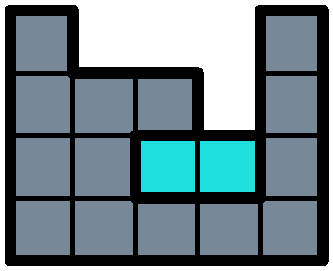
\includegraphics[width=0.9\textwidth]{pictures/dominoes/drs-1.pdf}
    \caption{}
  \end{subfigure}
  \begin{subfigure}[b]{0.2\textwidth}
    \centering
    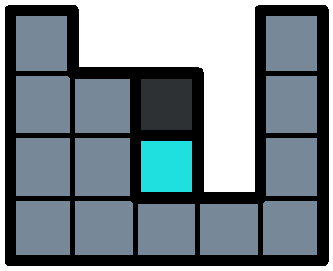
\includegraphics[width=0.9\textwidth]{pictures/dominoes/drs-2.pdf}
    \caption{}
  \end{subfigure}
  \begin{subfigure}[b]{0.2\textwidth}
    \centering
    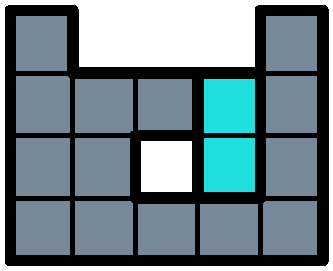
\includegraphics[width=0.9\textwidth]{pictures/dominoes/drs-3.pdf}
    \caption{}
  \end{subfigure}
  \caption{When rotating clockwise the domino in (a) DRS first ties to place it like (b), but this position isn't legal. Test 2 tries to place it in the right column which results a valid position.}
  \label{dom:drs}
\end{figure}

DRS let us move a piece freely through the board and also let pieces to move upwards in a staircase pattern as shown in Figure~\ref{fig:hola}. More importantly a domino can be placed almost anyway.

\begin{lemma0}
For any board configuration $B$, exists a trajectory that places a domino in any position reachable by any grid path that never goes vertically upwards.
\end{lemma0}
\begin{proof}
    Let $p = ( c_1,\dots ,c_k )$ be a that path. A path goes vertically at cell $c_l = \cell$ if $c_{l+1} = \cell[i+1][j]$ and $c_{l+2} = \cell[i+2][j]$, so no cell of $p$ satisfies that. Let's assume the domino is placed in cells $c_1$ and $c_2$. 


    Proving that given a domino placed in $c_l$ and $c_{l+1}$ there's a move, or a combination of moves, that places the domino in $c_{l+1}$ and $c_{l+2}$ the hole trajectory can be built. If $c_l$ $c_{l+1}$ and $c_{c+2}$ are in the same row/column, a slide/drop respectively the domino can be moved to the new position. The remaining cases are the turns. When the path passes throught filled cells, eight possible scenarios are in Figure~\ref{dom:turns}.

\begin{figure}[h]
    \centering
    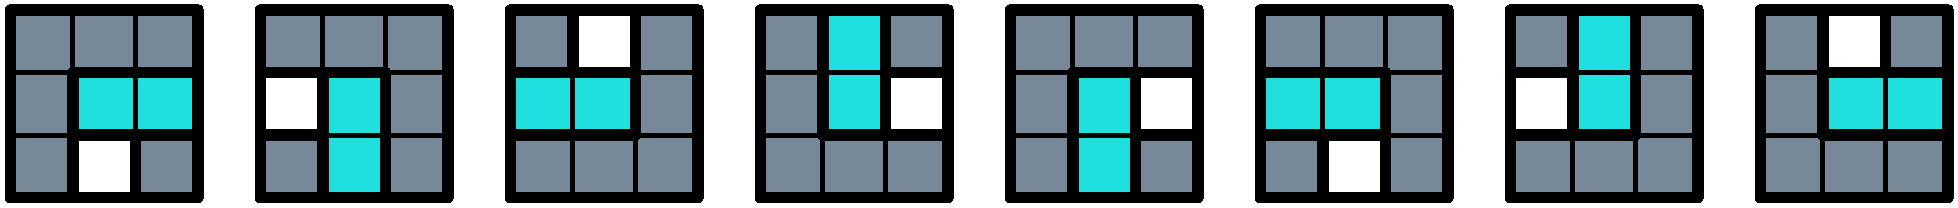
\includegraphics[width=\textwidth]{./pictures/dominoes/turns.pdf}
    \caption{The possible turns, in blue the domino and in white the destination cell.} 
    \label{dom:turns} 
\end{figure}

  The moves can be done respectively with: $r_-$, $r_-$, $r_+$, $r_+$, $r_+$, $r_-$, $r_-$ and $r_+$. In the first, second, fifth and eight turns DRS places the domino in the withe cells even directly, without any interfernce of surrounding cells. For the other moves the piece is placed in the corner, and the with a slide move the solution can be acomplished funnly.
\end{proof}


So a piece can be placed anyware of the baord except for the regions that can only be accesed thourhgt a vertiall path. An example of paths:

\textbf{dibuxet guai de camins}

We will divide the problem into two: deciding when the first row can be cleared and deciding when any other row can be cleared.


\begin{lemma0}
For any $n \times m$ board, deciding whether the top row can be cleared is in \pp.
\end{lemma0}
\begin{proof}
\end{proof}

\begin{lemma0}
For any $n \times m$ board, deciding if any row, except the first one, can be cleared is in \pp.
\end{lemma0}

\begin{proof}
  Let $B$ be a board in an initial configuration and $r$ the row to be cleared. To completely fill the row all its holes have to be filled. To place a domino inside the hole this needs to be reachable from the top of the board. Using previus lema we can see that a piece can be placed except for positions that can only be reached thorught verticall paths.

  Lets first consider the paths that reach the hole from the top. If a cell

\end{proof}
